\documentclass{article}
\usepackage{graphicx}
\usepackage{epsfig}
%\usepackage{pdflatex}
\title {SuperBigBite Data Acquisition Implementation}
\author{Alexandre Camsonne}

\begin{document}
\section{ Overview of experiments}
\subsection{Overview of neutron form factor experiments}
Both neutron form factor experiments measure quasi-free scattering on a nuclear target. The standard Hall~A
BigBite Spectrometer is used to detect the scattered electrons.  
Neutrons and protons are detected in
the hadron calorimeter (HCAL) which is located behind the Super BigBite Spectrometer Magnet. 
The Coordinate Detector (CDET) will be placed in front of the hadron calorimeter.
In the GEn experiment, the CDET will be used as a charge particle veto. In the GMn experiment,
the CDET will be used as a proton tagger. The trigger for the experiments will be the BigBite spectrometer 
signel arm electron trigger which is discussed in Section~\ref{sec:neutron-trig}.


Due to the increase in
luminosity, in comparison to earlier experiments, the tracking detectors (MWPC) need to be upgraded to
GEM chambers and the gas Cherenkov detector upgraded to a highly segmented 510 photo-multiplier gas
Cherenkov detector (known as the GRINCH).   The BigBite detector stack will consist of:
four GEM chambers (each covering 40x150 cm$^2$), the GRINCH gas cerenkov , one GEM chamber ( 60x200cm$^2$), 
scintillator paddle array, preshower and shower calorimeter. The scintillator array and preshower/shower
calorimeter will be unchanged from previous experiments. 

The preshower is 27 columns of two rows of lead glass which is placed perpendicular to the shower blocks.
The shower calorimeter consist of 27 rows and 7 columns of lead glass blocks. The 243 channels of
preshower and shower are readout in FASTBUS 1881M 64 channel ADC modules. The standard Bigbite 
scintillator array consists of one plane of scintillator paddles and can be used for the experiments. 
For the planned Hall~A $A_{1N}$ experiment, a 90  paddle scintillator array with
PMTs on both ends is being built the University of Glasgow. It is probable that it will
be ready for the SBS neutron form factor experiments, but it is not necessary for the experiments.

The 550 PMTs of the GRINCH gas Cherenkov detector will be input into 16 channel ampliflier/discriminator
cards based which use the NINO chip. The University of Glasgow has developed the cards and the cards have 
been bought. The logical output from the cards will be readout in FASTBUS 1877S 96 channel TDC modules.

The front 4 GEM chambers are being built by INFN group and are part of the total of six that
will be used as the front tracker for the proton form factor (GEp) experiment. Each chamber consists
of 3 GEM modules. Each GEM module covers an area of 40x50 cm$^2$. The readout plane is pitched at 400~$\mu$m
and is readout using 128 channel APV25 chips. Each module is readout by a total of 18 APV25 chips ( 8 along
the 40~cm and 10 along the 50~cm). So a GEM front chamber has 6912 channels which gives a total of 27648 channels
for the 4 GEM chambers. The APV25 chips will be readout by a VME64x/VXS Multi-Purpose Digitizer (MPD) that was
develop by an INFN group. It has been used in previous experiments. Details are given in Section.

The rear GEM chamber is being built by the University of Virginia and is part of the toal of 10 GEM chambers
that will be used as the rear tracker for the GEp experiment. Each chamber consist of 4 GEM modules.
 Each GEM module covers an area of 60x50 cm$^2$ and are combined into a chamber with an area
of 60x200 cm$^2$. The readout plane is pitched at 400~$\mu$m and two strips are combined to reduce
the number of readout channels. Readout is done using 128 channel APV25 chips. Each module is readout 
by a total of  12 APV25 chips (  6 along the 60~cm and 6 along the 50~cm). So a GEM rear chamber has  
6144 channels which gives a total of 61,440 channels for the 10 GEM chambers. The readout of the GEM
rear chamber APV25 chips will use the same INFN MPD electonics as the front GEM chambers.  
 
The hadron calorimeter, HCAL, is a 12x24 block array which will be readout 
by a JLab FADC250, a 16-channel 12-bit Flash 
ADC sampling at 250 MHz. For the neutron form factor experiments, the HCAL is not part of the trigger. For the
neutron form factor experiments, timing resolution is important at the 500ps level and the JLab FADC250 has 
demonstrated sub 300ps timing resolution. The FADC250 is readout through the VXS pipelined electronics
which is explained in Section~\ref{sec:hcal-vxs}.


The Coordinate Detector is  two planes of scintillator. Each plane consist of 1176 scintillator bars. 
Each scintillator bar is readout by a wavelength shifting fiber. Fourteen of the WLS  will be coupled to
a 16 channel multianode PMT. Each analog output of the PMT will be input to a 16 channel amplifier/discriminator
card base on the NINO chip. The logic signals from the NINO chip will go to FASTBUS 1877s 96 channel TDC modules.
Since the CDET is using only 14/16 channels , space is need for 2688 TDC channels ( 16/14*2352).
 


\subsection{Overview of proton form factor experiments}
\label{sec:over-pff}
The proton form factor, GEp, experiment measures elastic electron-proton scattering. For electron
detection, a large lead glass calorimeter, ECAL,  will be used with the Coordinate Detector, CDET, placed in front
of ECAL. The CDET is the same as used in the neutron form factor experiments except
that it will be arranged with one scintillator plane behind the other. The CDET is primarily used
to make a high precision measurement of the electron out-of-plane angle. The proton will be
detected in the SBS spectrometer which consist of front tracker INFN GEMs, a polarimeter and the HCAL.
The front tracker will consist of 6 INFN GEM chambers ( each GEM INFN chamber is 3 GEM modules of 40x50cm$^2$).
The polarimeter consists of two groups of 5 University of Virginia GEM chambers (each UVa GEM chamber
is 4 GEM modules of 60x50cm$^2$). The trigger will be a coincidence between the ECAL and HCAL.

The electronics for the front and rear GEM trackers will be the same as used in the neutron form factor 
experiments. The CDET electronics will be the same. The HCAL electronics will be still use the FADC250, but it will be part of the trigger. Details of the trigger are discussed in Section~\ref{sec:hcal-trig}.

ECAL is a large array of lead glass bars. In a previous proton form factor, GEp3,  experiment, 1784 lead bars
were used in a calorimeter which was a mixture of 1024 blocks with 3.8x3.8~cm$^2$ cross sectional area and
760 blocks with 4x4~cm$^2$ cross sectional area. A larger pool of the same size lead glass bars is 
available at Jefferson Lab.
The electronics and cabling from that experiment will be re-used. The 
lead glass bars will be readout out by  FASTBUS 1881M 64 channel ADC modules. As done in the GEp3 experiment,
the analog signals from 8 blocks will be summed together in groups of 2x4 using custom built ``summing'' modules.
The ``summing'' modules have two sets of eight inputs. Each set of eight inputs is summed together
and six summed analog outputs for each group of eight are available. In addition the ``summing'' module 
produces the 16 individual
analogs signal with an amplification of 4.2 that can be sent to an ADC. The amount of electronics is
estimated assuming a block size of 4x4~cm$^2$. Under this assumption, one needs 1776 blocks and would 
have 214 ``group of 8'' sums. One of   ``group of 8'' analog signals would be sent to a discriminator 
and then a FASTBUS 1877S TDC. Other analog outputs from the  ``group of 8'' would be sent to additional
FI/FO units to form summed analog signal from a group of 32 blocks to be used in the ECAL trigger as
explained in Section~\ref{sec:ecal-trig}.

 


\subsection{Detector configuration summary}
\begin{tabular}{|c|c|c|c|}
\hline
GEp Detectors & Channels& Readout & Type \\
\hline
\underline{SBS Proton arm} & & & \\
Front tracker (6 GEM chambers) & 41,472 & APV25 MPD& VME\\
Rear tracker (10 GEM chambers) & 61,440& APV25 MPD& VME\\
HCAL & 288 & FADC 250 &VME\\
\hline
\underline{Electron arm} & & & \\
ECAL & 1776 & ADCs 1881M &Fastbus\\
ECAL sums& 214 & TDCs 1877S &Fastbus\\
CDET & 2688 & TDCs 1877S &Fastbus \\
\hline
\hline
GEn/GMn Detectors & Channels& Readout & Type \\
\hline
\underline{SBS Proton arm} & & & \\
HCAL & 288 & FADC 250 &VME\\
CDet & 2688 & TDCs 1877S&Fastbus\\
\hline
\underline{BigBite Electron arm} & & & \\
PreShower/Shower & 243 & ADCs 1881M&Fastbus\\
Scintillator & 180& ADCs 1877S&Fastbus\\
Gas Cerenkov & 550& ADCs 1877S&Fastbus\\
Front Tracker (4 GEM chambers) & 27648 & APV25 MPD &VME\\
Rear Tracker (1 GEM chamber) & 6144& APV25 MPD &VME\\
\hline
\end{tabular}

\section{Trigger}
\subsection{Neutron form factor experiments}
\label{sec:neutron-trig}
The shower calorimeter consist of an 7x27 array of  lead glass blocks. A preshower
 layer of 2x27 is placed in front of the shower
An analog sum of 7 blocks is made. This sums are further added using 4 channels linear fan module.
A preshower layer 2x27 is placed in front of the shower but is usually 
used off line for pion electron identification. 
This make a total of 189 + 54 = 243 lead glass blocks to be readout.
The readout of the detector will be done using fastbus using ADCs 1881M.
 The trigger for the neutron form factor experiments will use the 
standard electron trigger using the preshower and shower calorimeter which was developed for previous experiments. 
For the quasi-free kinematics of the experiments, the trigger provides sufficient pion rejection to keep the
trigger rate below 5 KHz. There is a side project to include the gas cerenkov in the trigger, but this
is not necessary for the experiments and the main focus is for the A$_{1N}$ experiment .

\subsection{Proton form factor experiments}
The trigger is a coincidence between the electron calorimeter, ECAL,  and the hadron calorimeter, HCAL.
Both ECAL and HCAL each form a trigger separately. Then a coincidence between the two is made which
takes into account the elastic angular correlation to reduce backgrounds.

\subsubsection{ECAL trigger}
\label{sec:ecal-trig}
 In the right   figure, the groups of 32 blocks are indicated connecting
group of 8 blocks by different colored squares. The group of 32 blocks overlap
by two groups of 8 in both horizontal and vertical directions. So most of the
groups of 8 have to go to 4 groups of 32. At the edges the groups of 8 feed into
two groups of 32. There are 228  groups of 32 are sums of 4 groups of 8 using
a 4 input channel linear FI/FO. The 228 groups of 32 would have to
go into discriminators.


\begin{figure}
  \centering
  % Requires \usepackage{graphicx}
  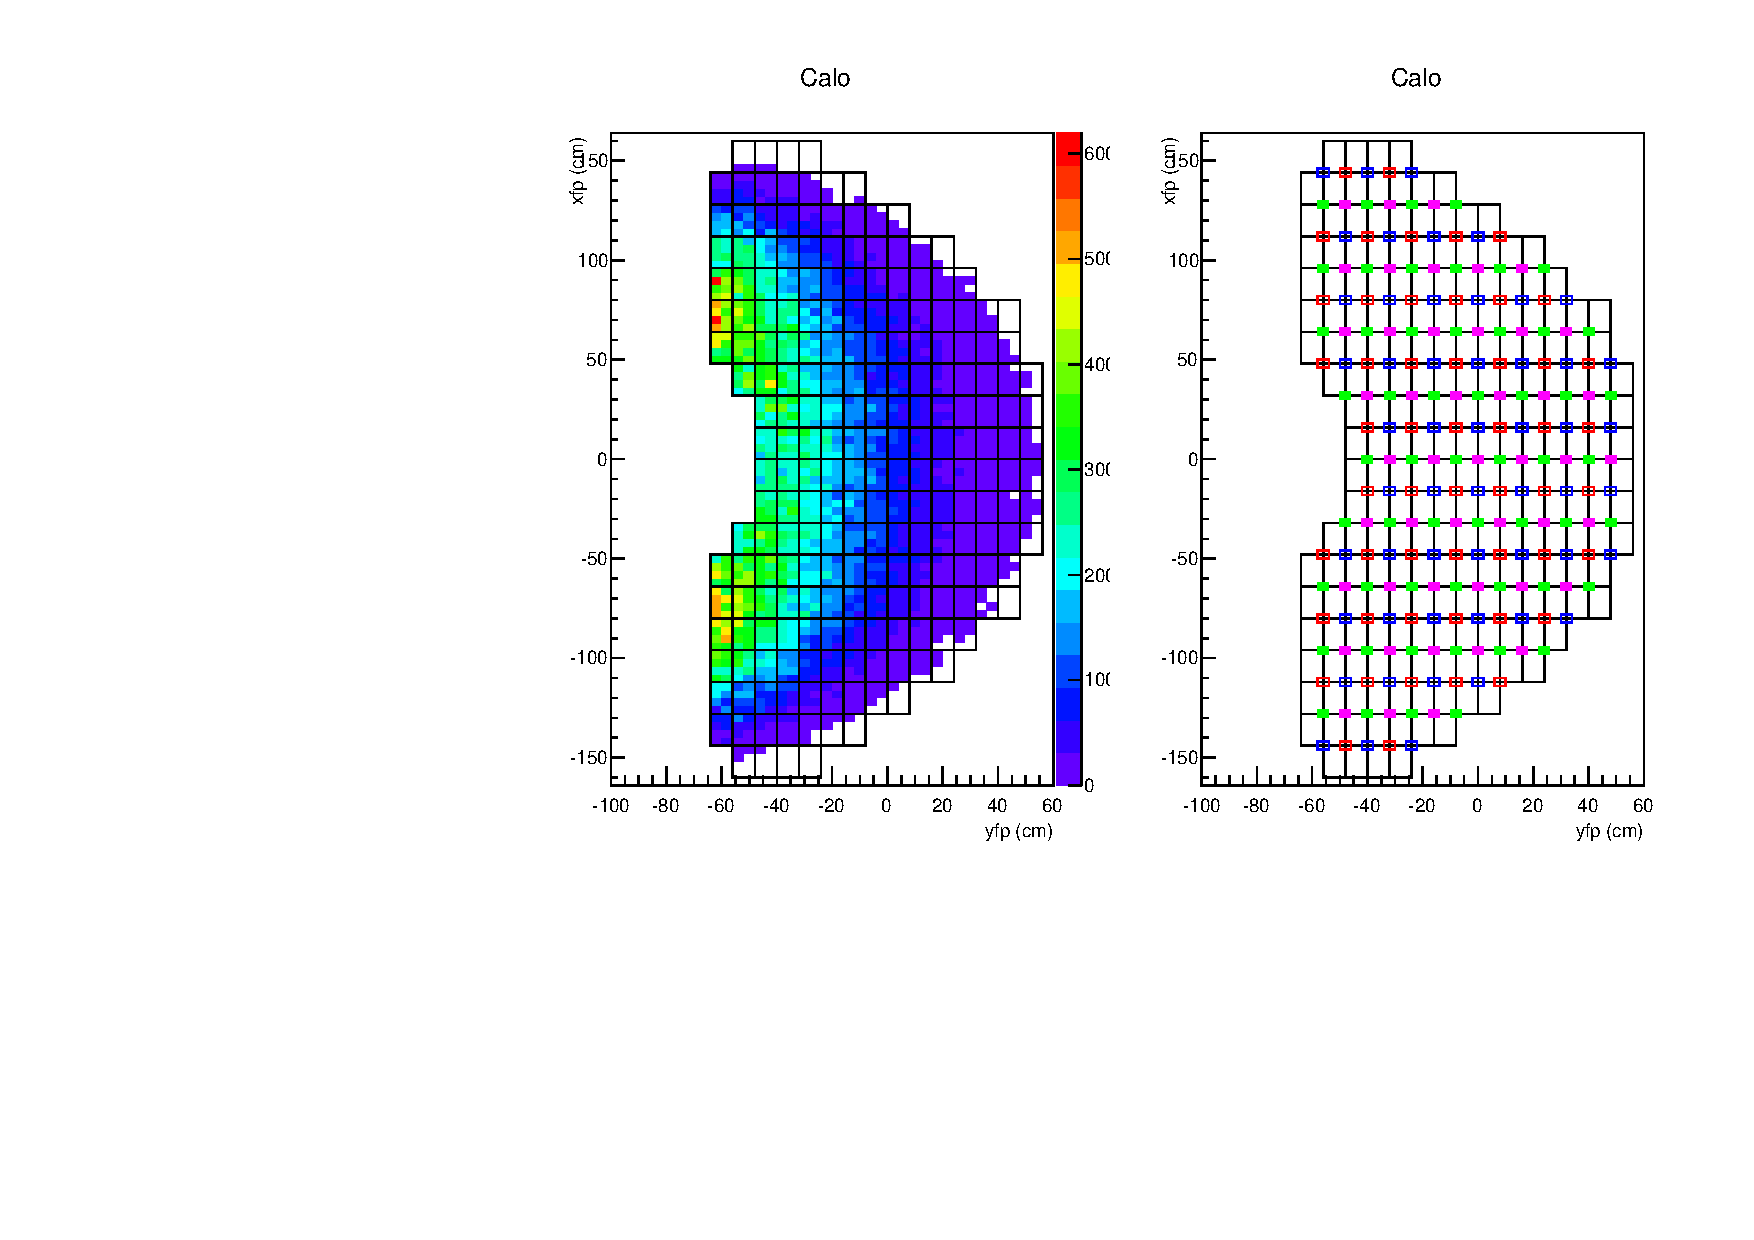
\includegraphics[width=\textwidth]{figs/cfpa.pdf}\\
  \caption{The left plot is the distribution of elastic electrons in ECAL with the black rectangles representing
groups of 2x4 lead glass blocks. The right plot demonstrates
the scheme for make overlapping groups of 32 lead glass blocks to be used in the ECAL trigger with
details explained in text.  }\label{fig:ECALTrig}
\end{figure}

\subsubsection{HCAL trigger}
\label{sec:hcal-trig}

In parallel the Hadron calorimeter is readout and a proton single trigger will be generated.
The rates expected in the calorimeter

\newpage

\section{DAQ Details}
\subsection{CODA}
\subsubsection{Introduction}
Jefferson Laboratory is using the Cebaf Online Data Acquisition system for data taking.
CODA is based on a main server interacting with a database in which all the DAQ components update their status . The readout crates host a single board computer running a Read Out Controller (ROC) program which controls and reads out the data from the electronics. The ROCs send the data through a standard network link usually ethernet to a computer running the Event Builder program, which uses the data from the ROC to check synchronization and build the event. Finally the event is sent to the Event Recorder which puts the event into a file on the hard drive of the computer.
\subsubsection{CODA Hardware}
In addition to the software a set of harware components specific to CODA is used in order to keep ensure event synchronization between all the components each crate has a trigger interface ( TI board ) which sends the trigger signal to the ROC program for the read out of the data. All the TI are linked to a trigger supervisor board which takes the triggers and sends them to the TI while monitoring the status of each TI to keep all the crates synchronized and generates a Level 1 accept and Level 2 accept for the read out modules. The TS also takes as input the front end busy of the modules to inhibit the triggering if one module is not ready insuring synchronization between the modules.
This allows the TS module to buffering if the front-end has the capability. The triggers and read out are then decorrelated which improve the deadtime since a module can take triggers while being readout asynchronously. The TS has a setting of the maximum of events which can be in the buffer it is set to the smallest buffer available on the electronics ( usually 5 for fastbus ). Since in this mode modules can potentially get out of synchronization, a synchronization event is set so that when a certain number of triggers is processed, the TS will disable the triggers to empty the FIFO. If there any remaining events in the FIFO a warning issue would be issued and the FIFOs would be cleared resynchronizing the modules.
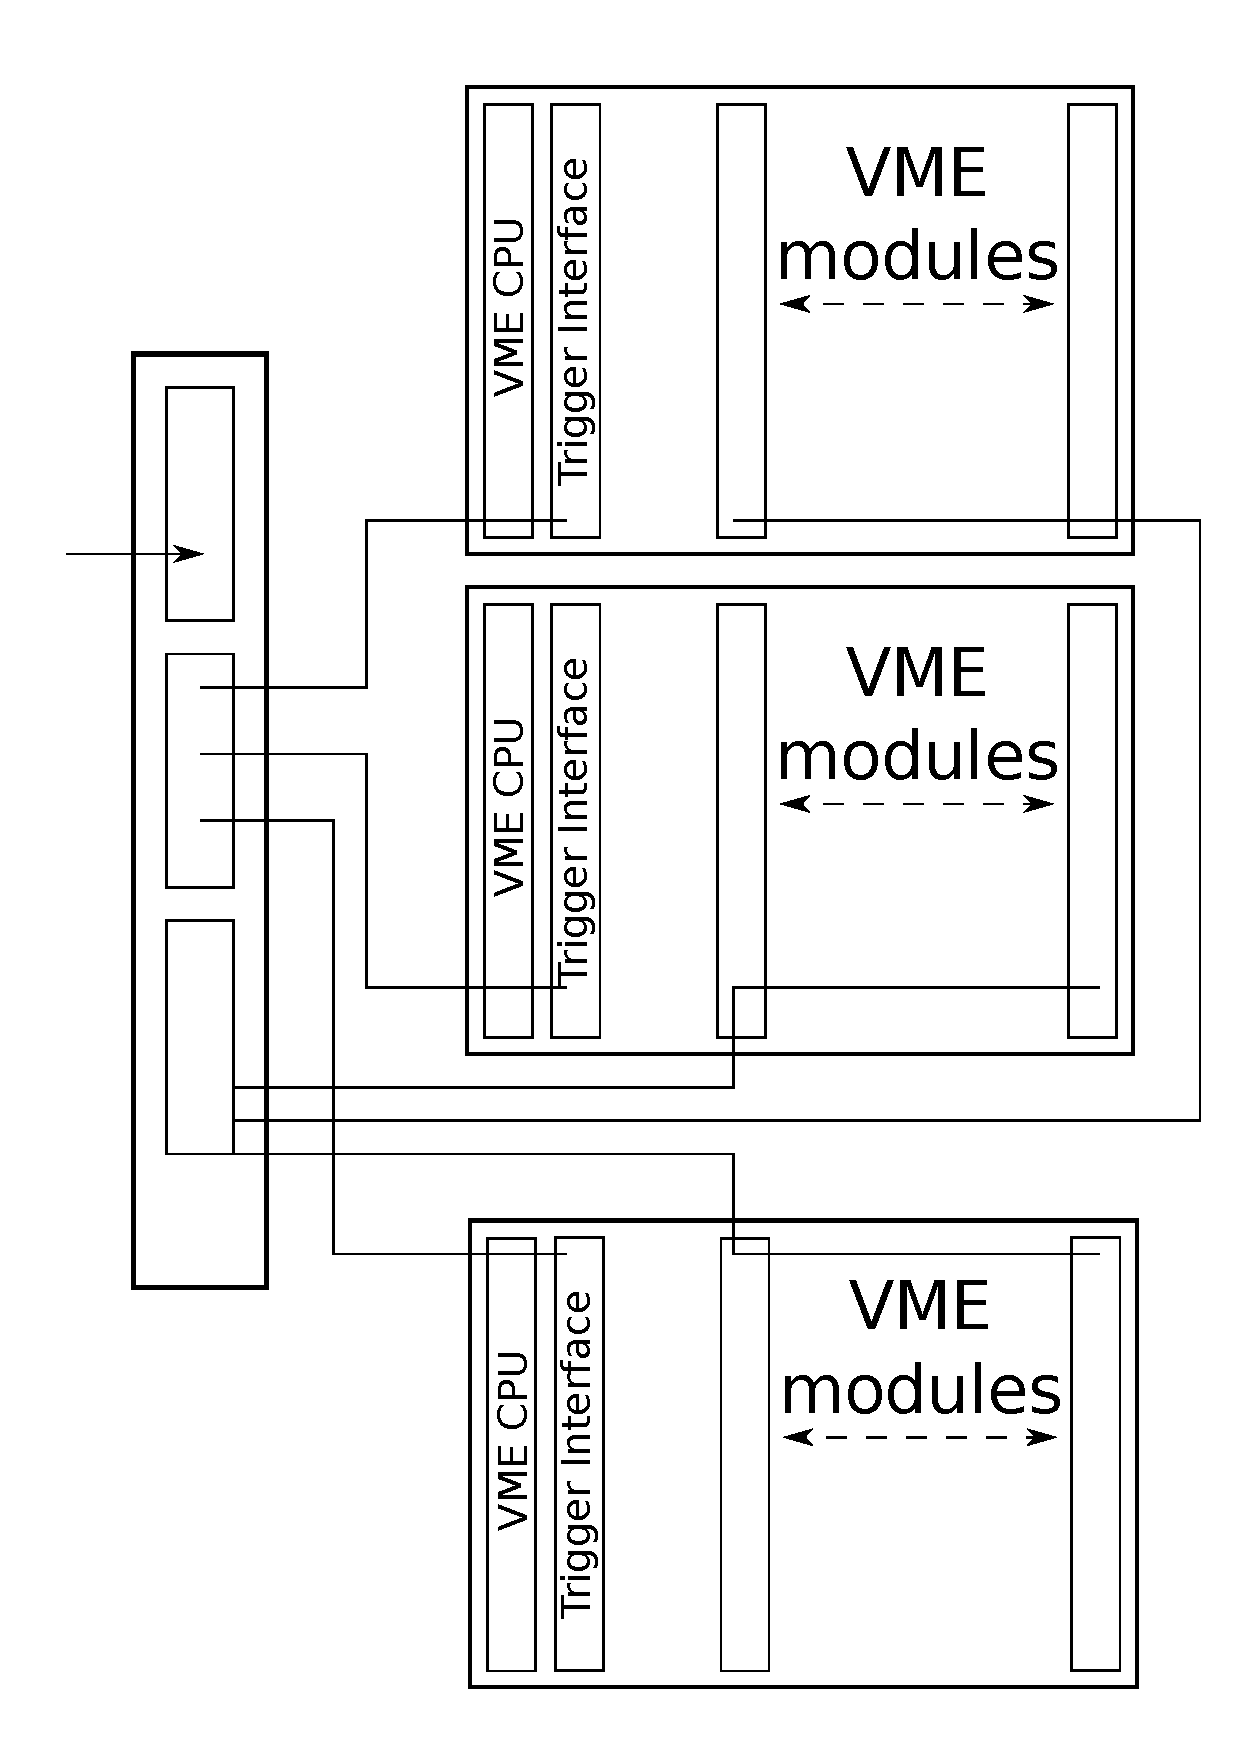
\includegraphics[scale=0.55]{figs/TS.pdf}\\
  

\section{Electronics}
\section{GEM readout}
The GEM readout is carried out by the APV25 chip. It a pipelined ASICs with 128 channels and pipeline depth of 192 samples sampling at 40 MHz. When a trigger is issued the corresponding cells are frozen until they are readout while the other cells are still being used reducing the dead time.
For each trigger all the data of 128 channels are transfered at 40 MHz rate in a multiplexed analog format. Adding some header and event informations 141 words are transmitted for each trigger which gives a transfer time of $141x25 ns = 3.6 \mu s $. In case of high background several consecutives time samples can be sent in order to detect pile up, we plan to read 3 samples which gives a transfer time of 10.8 $\mu s$. This allows deadtimeless operation for rates up to 90 KHz. The readout planned to be use the the INFN Multi Purpose Digitizer (MPD), it is a VME board with a 200 MHz FADC and signals to control the APV setup and readout. 


\section{Pipelined electronics, HCAL trigger}
\label{sec:hcal-vxs}
The hadron calorimeter will be read out by the JLAB pipelined electronics.
The central module for this system is the JLAB FADC250, a 16-channel 12-bit FADC sampling at 250~MHz. The input signals are continuously recorded into the memory with a memory depth up to 8 us. The system is thus dead timeless as long as the trigger is generated before the memory rolls over and the event of interest is overwritten.
The Flash ADC has two separated data path.
The first one uses the new high speed serialized VME standard called VME switched Serial (VXS).
It allows full duplex point to point connection at up to 2.5 Gbps per lane using the backplane central connector.
Currently the FADC is using two VXS lanes giving 5 Gbps of bandwidth.
This allows to transfer a 16 bit word from each FADC to a Crate Trigger Processor (CTP) board every 4~ns.
Each FADC being connected to The CTP via a 5 Gbps link, the CTP uses up to 16 FADC words from each FADC to form a 32-bit word every 4~ns which can be a lower resolution sum of all the channels or a bit pattern of the channel hit for example.
The CTP board then sends the processed signals to a Sub-System Processor (SSP) board via a 10 Gbps optical link which puts together all the data from individual crates and computes the associated quantities which will be used in the trigger.
All the SSP boards send their processed information to a Global Trigger Processor (GTP) which makes the L1 trigger.
The GTP sends the trigger to the Trigger Supervisor (TS) which makes sure the system is ready to accept a trigger and sends the accepted signal to the Trigger Distribution boards in the VXS crates which are linked to the Trigger Interface boards in each crates via optical link as represented in Fig.\ref{fig:pipeline_daq}.
The trigger and synchronization clock signals will then be sent back to individual crates and payload modules through Trigger Interface/Distribution (TID) boards and Signal Distribution (SD) boards which distributes the signals to the electronics such as the FADC.
Once a trigger is generated, the full resolution data which is still in the pipeline is readout out using the VME320 protocol at an average data rate of 200 MB/s.
The Flash ADC can run in different modes, it can either transfer all the samples of the waveform which can be useful to study pileup effect and background or process the data to give an integral over the length of the pulse.

\begin{figure}
  \centering
  % Requires \usepackage{graphicx}
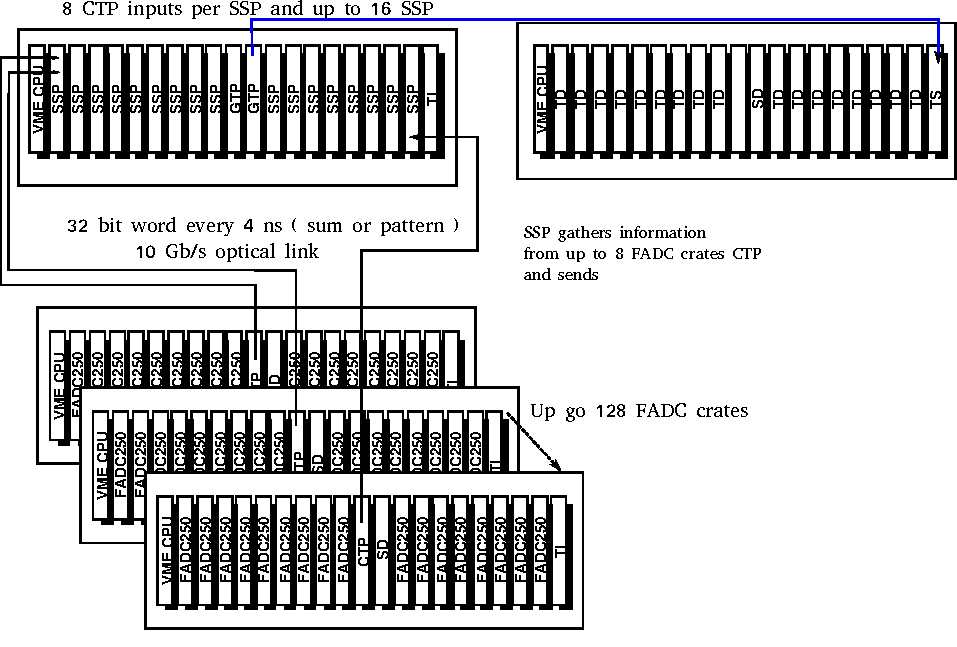
\includegraphics[width=\textwidth]{figs/TriggerPipeline.pdf}\\
  \caption{Standard Triggering scheme using the JLAB pipeline electronics}\label{fig:pipeline_daq}
\end{figure}

The CTP having all the amplitude of all the calorimeter, it can compute all the sums of adjacent blocks.
A sum of 3$\times$3 blocks was implemented.
In order to reduce the number of triggers coming from the background this summing approach is chosen to improve the online pion rejection.
A sum over 1 central block and 6 surrounding blocks can be implemented in the same way as the HPS scheme.

\begin{figure}
  \centering
  % Requires \usepackage{graphicx}
 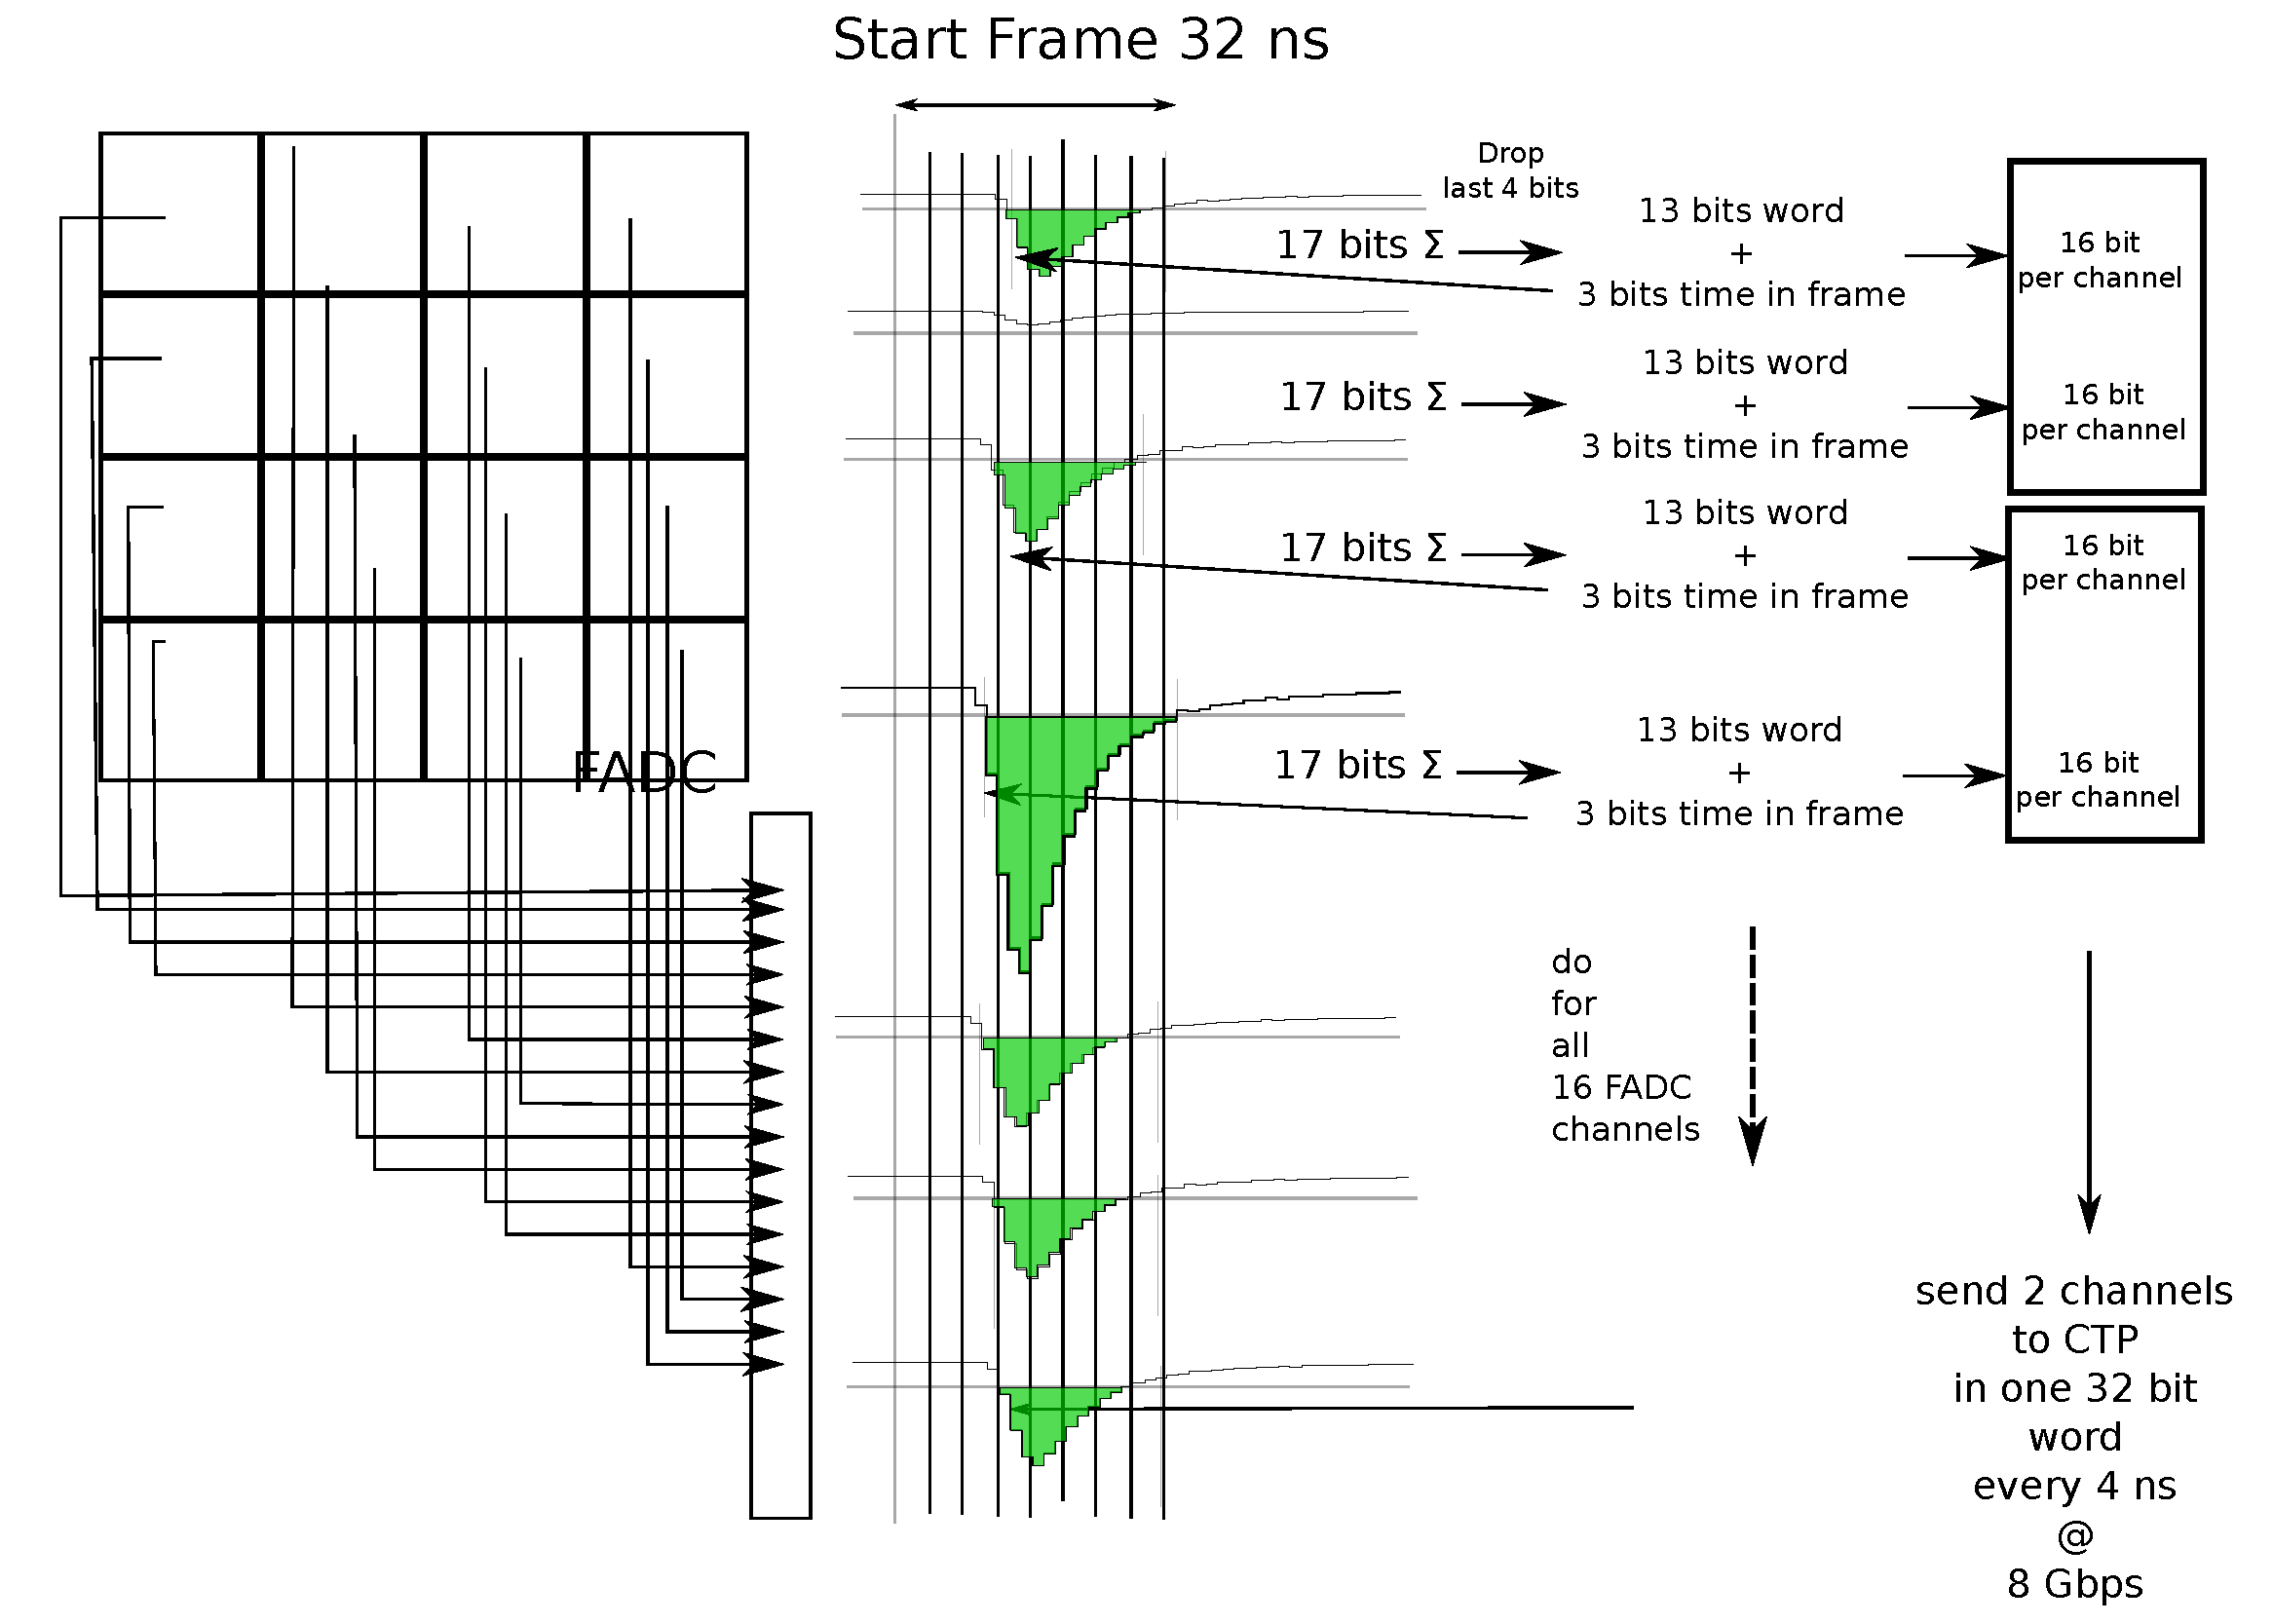
\includegraphics[width=\textwidth]{figs/CaloTrigger.pdf}
  \caption{Calorimeter clustering scheme using the HPS algorithm. All calorimeter signals are sent to the FADC. }\label{fig:ClustHPS}
\end{figure}

\begin{figure}
  \centering
  % Requires \usepackage{graphicx}
 %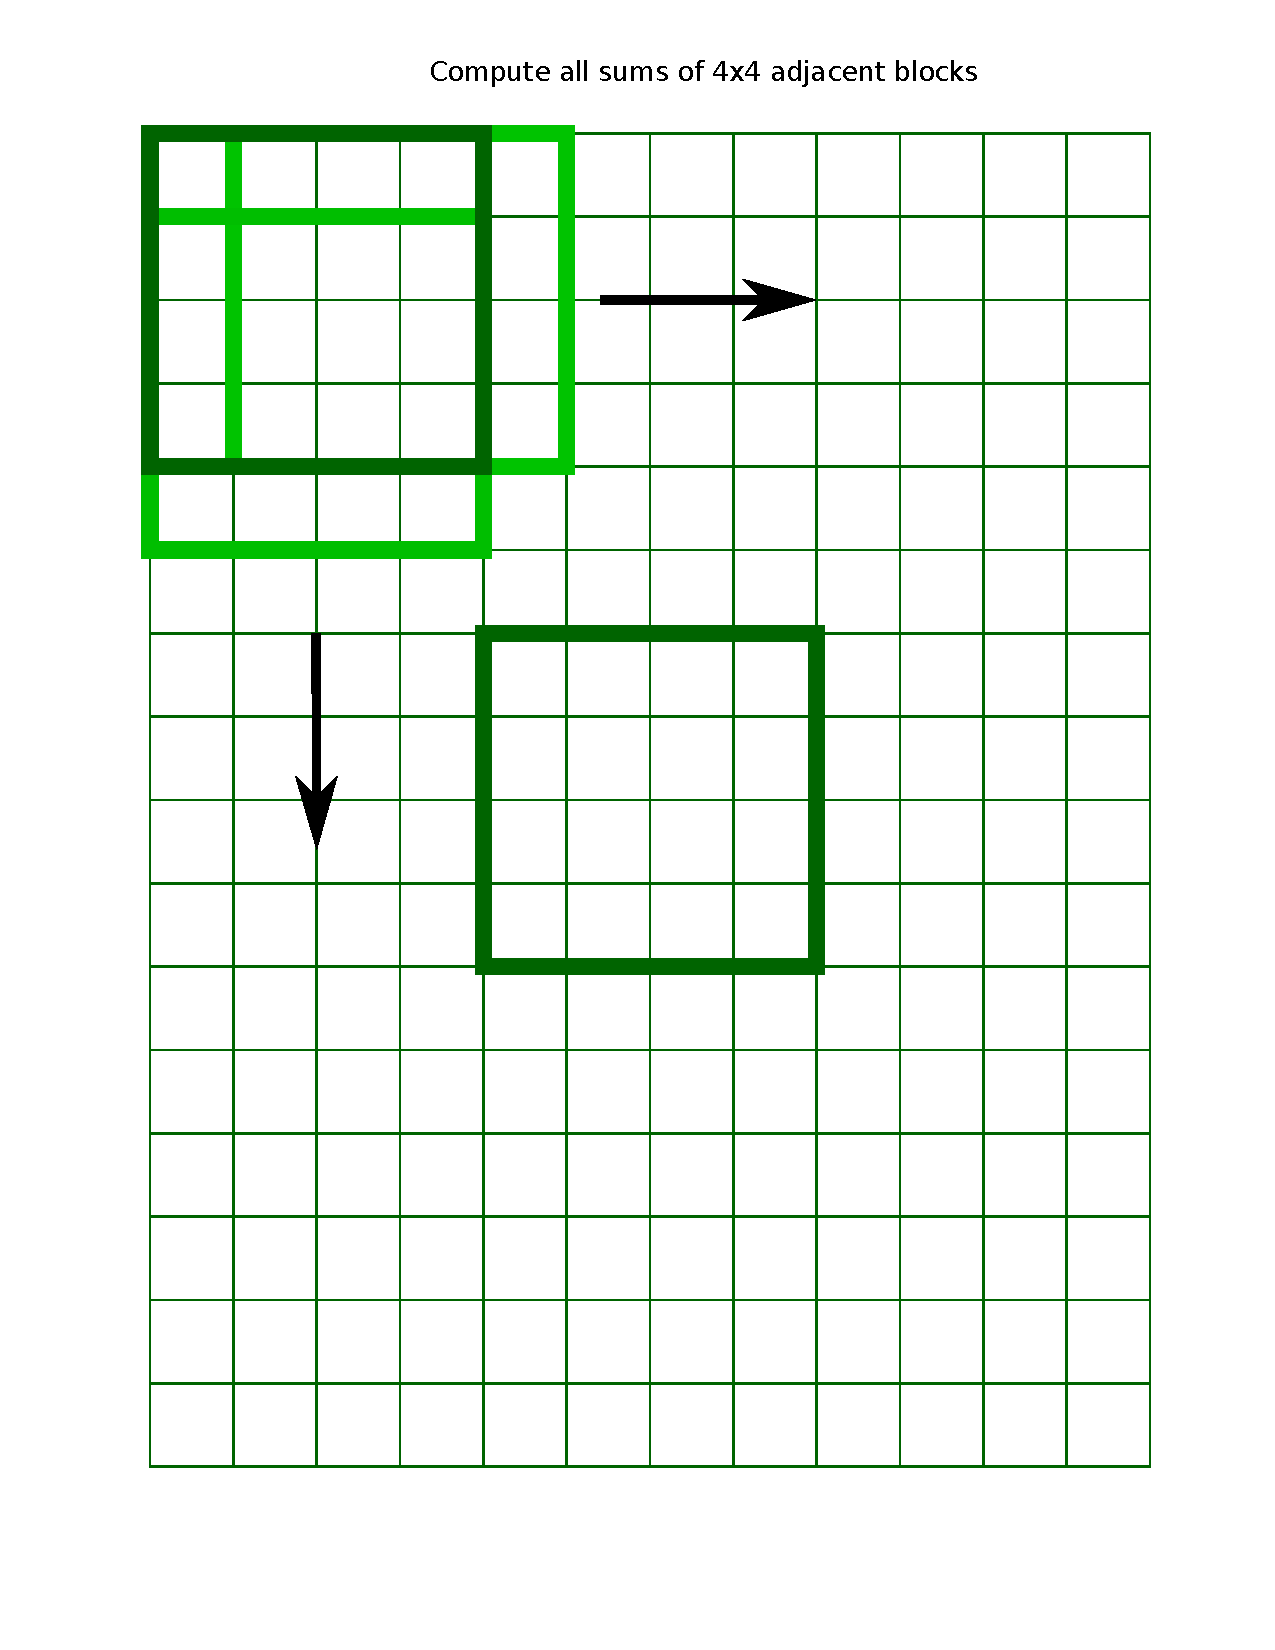
\includegraphics[width=\textwidth]{figs/HCALSum.pdf}
  \caption{All sum of 4x4 are computed, if one is above threshold L2 is generated }
\end{figure}

\begin{figure}
  \centering
  % Requires \usepackage{graphicx}
  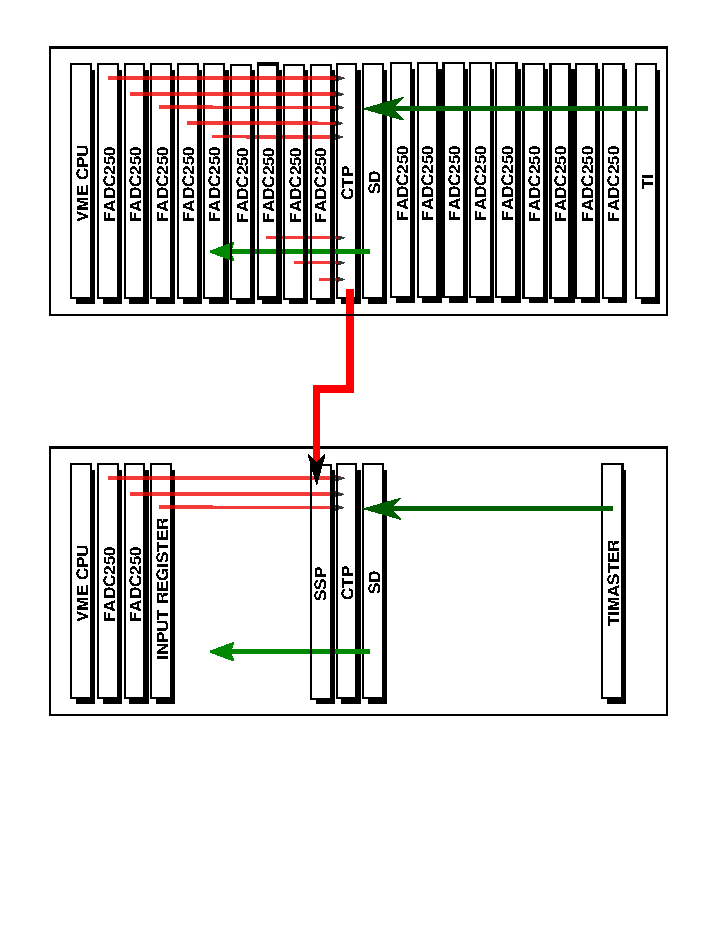
\includegraphics[width=\textwidth]{figs/VXSHCalFADC.pdf}\\
  \caption{HCAL crate layout }\label{fig:HCALFADC}
\end{figure}

\section{Fastbus}
Fastbus is an electronics standard . It can transfer up to 10 Megawords per second with a 32 bit width which gives a maximum theoretical throughput of 40 MB/s which translates in usual sustained rate of 15 MB/s.
Since we have a lot of Fastbus equipment on hand. It will be used in order to save money for the large number of detectors channels. The main readout is the Lecroy ADC 1881M a 13 bit ADC, with a 9 $\mu$s encoding time in 12 bit resolution and 12  $\mu$s. The 1881M features a fast clear and is ready to tahe another event after 1 $\mu$s. For signal requiring time measurement 1877S TDC will be used, they have 96 channels per module. It is multihit with an event buffer of 8 events. It has an encoding time  1.7 $\mu$s plus 50 ns per hit per channel giving a maximum encoding time of 78 $\mu$. 
The Struck Fastbus Interface is a Fastbus Master is controlled by a standard VME controller which allows to control the Fastbus modules through any VME CPU. It is needed in each Fastbus bin to control the Fastbus modules.

\begin{tabular}{|c|c|}
\hline
&\\
\hline
&\\
\hline
\end{tabular}






\newpage
\begin{figure}
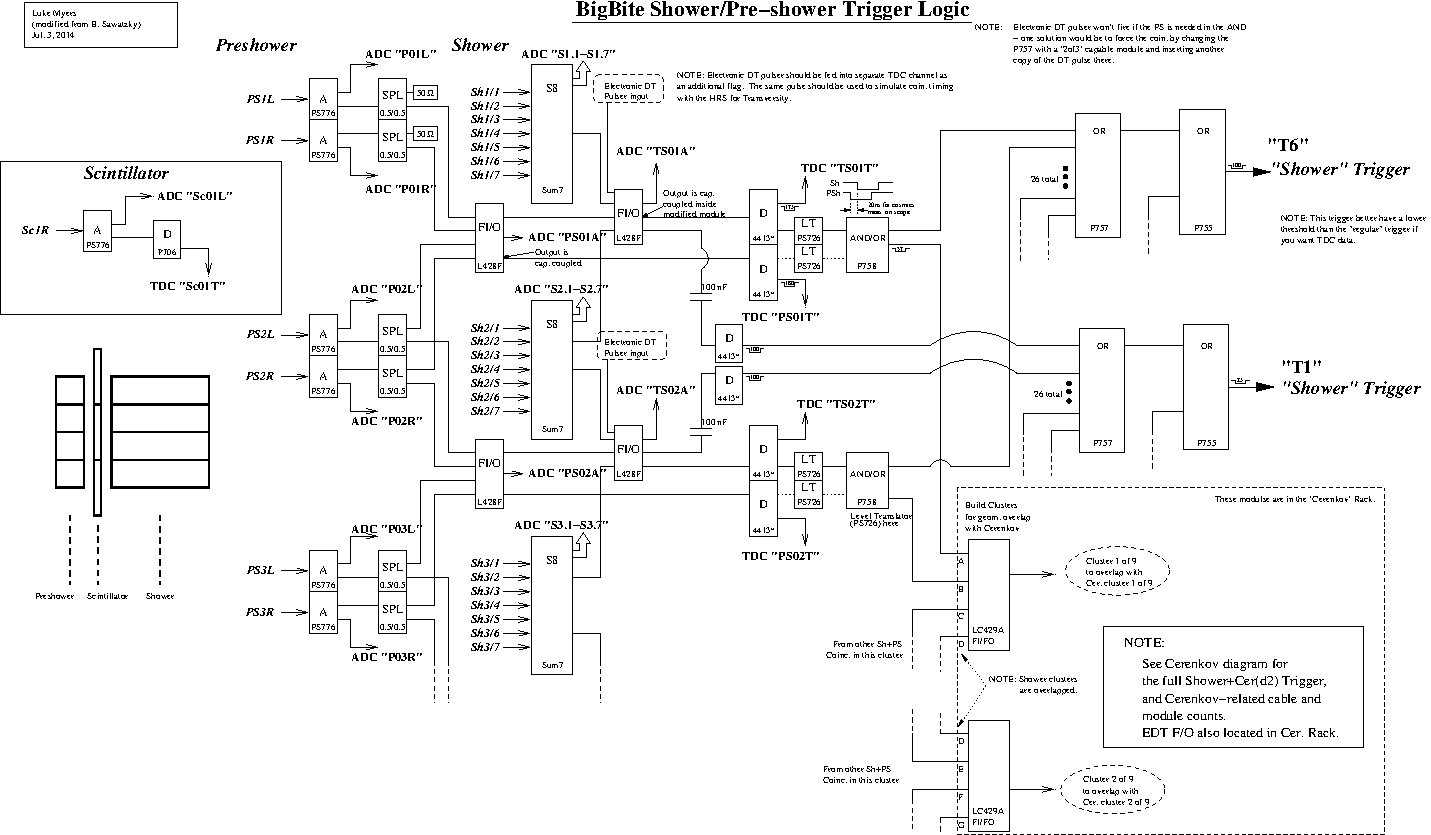
\includegraphics[scale=0.9,angle=270]{figs/Sh-PS_logic_v2A.pdf}\\
\caption {BigBite electron shower analog sum trigger \label{BBEtrig}}
\end{figure}
\newpage









\subsection{Readout}

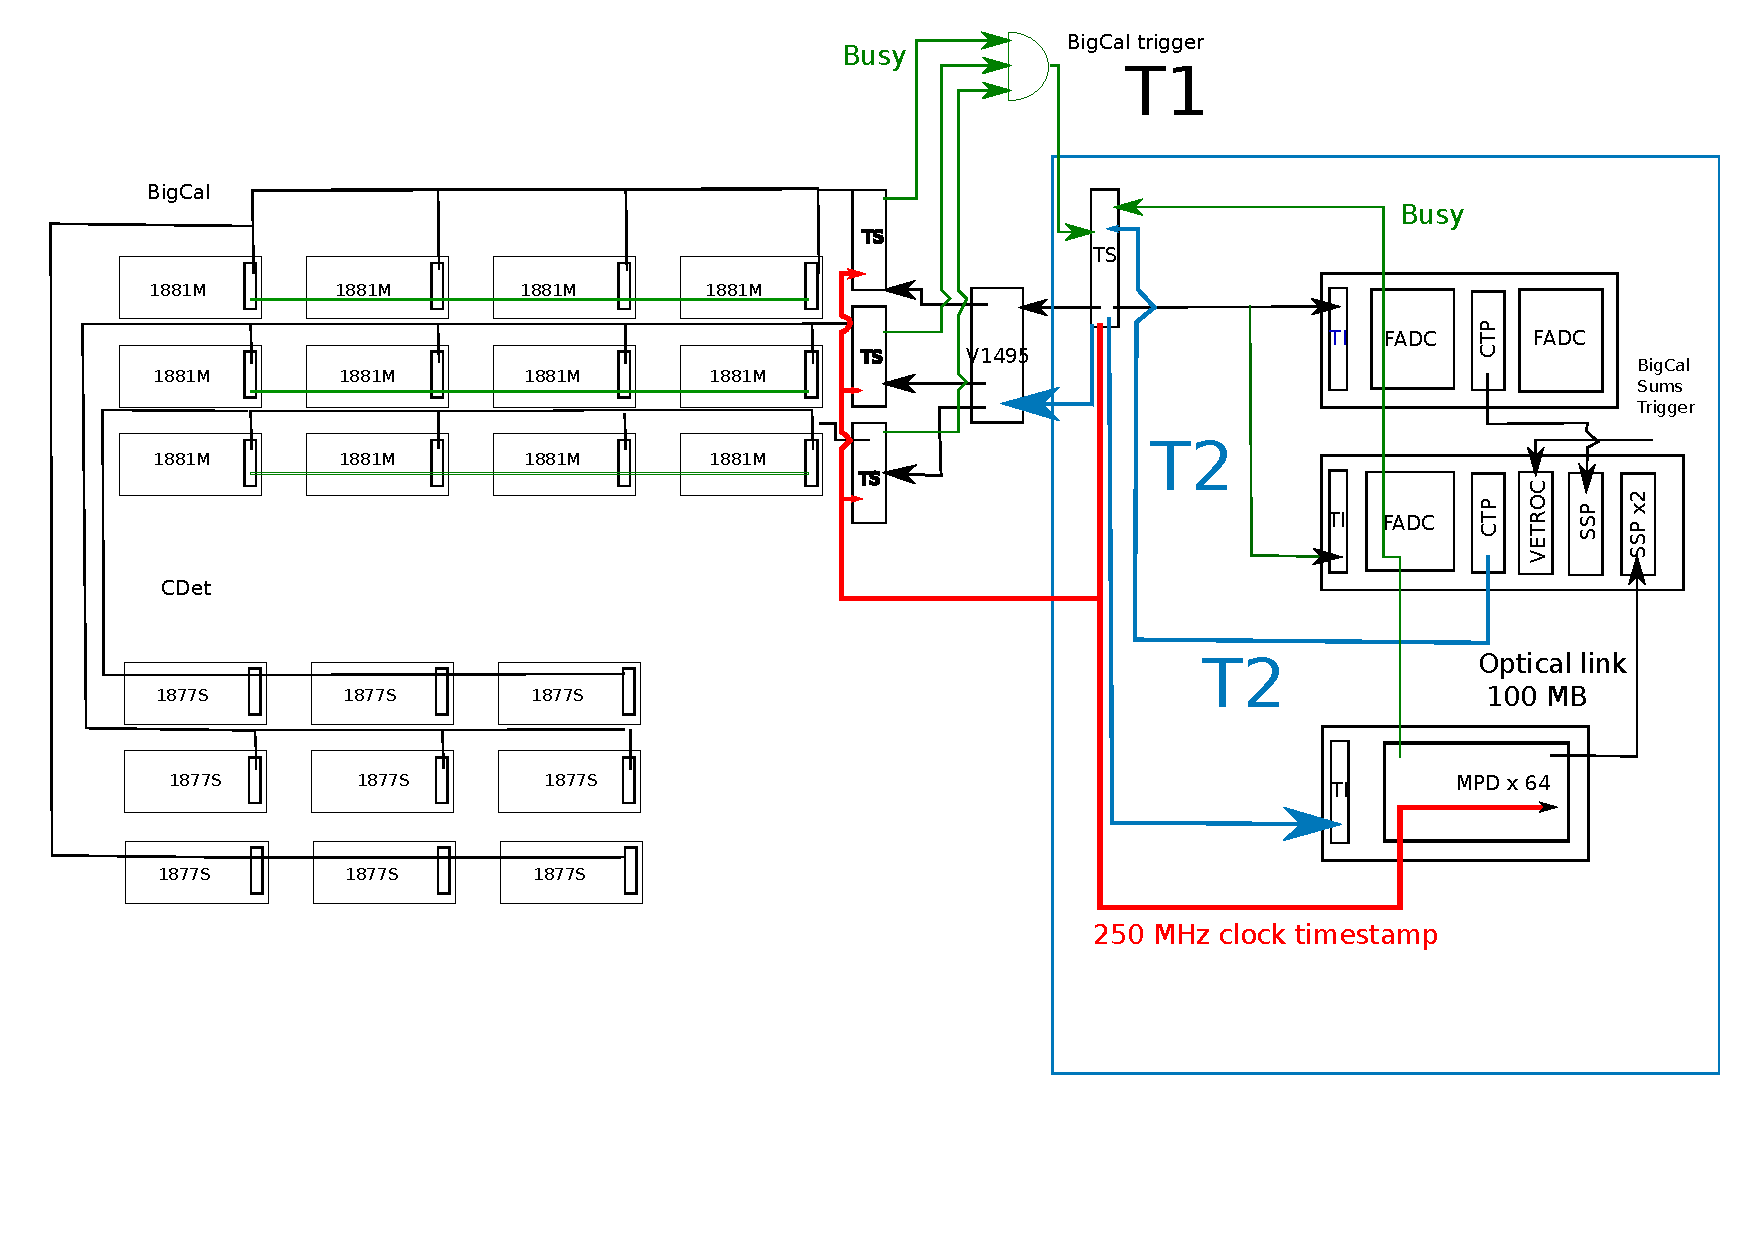
\includegraphics[scale=0.55]{figs/SBSlayoutOld.pdf}\\


\subsection{Event size and data rates}
\section{Data acquisition for GEn experiment}

PR-09-016 GEN
about 2 kHz from a simulation based on pion production rates from a parameterization done by
Wiser [69], Fig. 22. This simulation when compared to the previous Gn
E experiment predicted rates
higher by a factor of 5, so this produces an upper limit on expected rates. Furthermore, adding the
Cerenkov into the trigger configuration to explicitly reject pions and photons will be possible if
necessary


\subsection{Requirements}
\subsection{Detectors}
\subsection{Trigger}
The trigger will be single quasielastic electron in BigBite.
The expected trigger rate at high Q2 is low even without having the Gas Cerenkov in the trigger.
In case of unforeseen background, the same scheme as GEp5 could be used by using a L1 and L2 trigger from HCAL for a neutron trigger
to have a coincidence between the two arms.
\subsection{Readout}

\subsection{Event size and data rates}
\section{Data acquisition for GMn experiment}
Comparing those thresholds
to Fig. 23 shows that the expected background trigger rates are comfortably low, generally well
below 1 kHz.

Q2 3.5 4.5 6.0 8.5 10. 12. 13.5 16. 18.
Quasi-elastic E’min (GeV) 2.4 1.8 1.1 1.8 3.0 2.0 1.4 2.1 1.2
Threshold (GeV) 2.1 1.6 1.0 1.6 2.7 1.8 1.2 1.9 1.0



\subsection{Requirements}
\subsection{Detectors}
The configuration is similar to the GEn experiment except for calibration run using the RHRS.

\subsection{Trigger}

\subsection{Readout}

\subsection{Event size and data rates}

\begin{thebibliography}{9}
\bibitem{GEnProp} PR
\bibitem{GEpProp} PR
\bibitem{GMnProp} PR
\bibitem{TransProp} PR
\end{thebibliography}
\end{document}
